\section{Code design and implementation}
\label{sec:code}
\CC{} -- abstraction, encapsulation, inheritance and polymorphism


Instead of making separate classes for capacitors, inductors and resistors, an abstract base class was made which functions as an interface for all three. The RCL classes then inherit from this class This abstract base class, \verb!Component!, contained a virtual function prototype \verb!get_impedance! which is


\CC{} allows programs to be broken up into multiple files in a bid to reduce the number of lines per file and make the code more readable and more straightforward for the programmer to edit. Separating classes into a separate file allows for modularity; that is the ability to reuse the same classes for different programs.
A further feature of this modularity is the ability to separate the interface of each class from its implementation. By separating the interface into a header file (many conventions exist for the naming of \CC{} header files but this project exclusively uses the \verb!.h! extension) and consists of the class definition in which the member data are declared and the member functions are prototyped. Header files are included (with the \verb!#include "*.h"! preprocessor directive) but not compiled, whereas source files are compiled but not included. The implementation was contained in files with the \verb!.cpp! extension, but like header files, many other naming conventions exist.


In the design of this project, the code was split into seven header files which contained class definitions, namespace and seven source files which are listed along with a short description of their contents.

\begin{figure}
  \begin{center}
    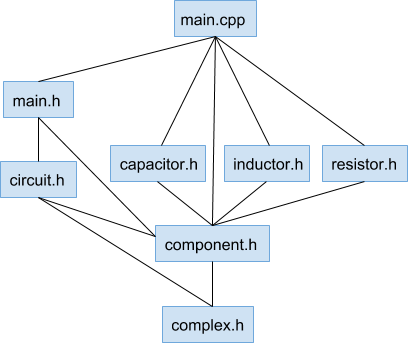
\includegraphics[width=.5\textwidth]{hierarchy}
  \end{center}
  \caption{The hierarchy of header files showing the main file at the top and the chain of its dependencies leading down.}
  \label{fig:hierarchy}
\end{figure}

%\subsection{\CC{} concepts}








prototyping functions\\

vectors\\
smart pointer\\
lambdas\\
namespaces and binary scope operator\\
function template\\
static data\\
